\documentclass{article}

\usepackage[italian]{babel}
\usepackage[margin=2cm, footskip=5mm]{geometry}
% questi package non sono necessari in lualatex; ref https://tex.stackexchange.com/a/413046
% \usepackage[utf8]{inputenc}
% \usepackage[T1]{fontenc}
\usepackage{enumitem}
\usepackage{hyperref}
\usepackage{titlesec}
\usepackage{soulutf8}
\usepackage{contour}
\usepackage{float}
\usepackage{graphicx}
\usepackage{fancyhdr}
\usepackage{longtable}
\usepackage[table]{xcolor}
\usepackage{titling}
\usepackage{lastpage}
\usepackage{ifthen}
\usepackage{calc}
\usepackage{minted}
\usepackage{pgfgantt}
\usepackage{subfiles}

\newlength{\imgwidth}

\newcommand\scalegraphics[1]{%
    \settowidth{\imgwidth}{\includegraphics{#1}}%
    \setlength{\imgwidth}{\minof{\imgwidth}{\textwidth}}%
    \includegraphics[width=\imgwidth]{#1}%
}

% XXX definizione dei percorsi in cui cercare immagini
\graphicspath{ {./}
    {./img/}
}

% esempio di utilizzo: \appendToGraphicspath{./img/} (un comando diverso per ogni path da includere)
% N.B.: ci DEVE essere un forward slash alla fine del path, a indicare che è una cartella.
\makeatletter
\newcommand\appendToGraphicspath[1]{%
  \g@addto@macro\Ginput@path{{#1}}%
}
\makeatother

% setup della sottolineatura
\setuldepth{Flat}
\contourlength{0.8pt}

\newcommand{\uline}[1]{%
  \ul{{\phantom{#1}}}%
  \llap{\contour{white}{#1}}%
}

% setup dei link
\hypersetup{
  colorlinks=true, % set true if you want colored links
  linktoc=all,     % set to all if you want both sections and subsections linked
  linkcolor=black, % choose some color if you want links to stand out
}

% setup di header e footer
\pagestyle{fancy}

\fancyhf{}
\fancyhead[L]{\includegraphics[width=1cm]{logo.png}}
\fancyhead[R]{\thetitle}
\fancyfoot[R]{\thepage\ di~\pageref{LastPage}}

\fancypagestyle{nopage}{%
  \fancyfoot{}%
}

\setlength{\headheight}{1.2cm}

% setup forma \paragraph e \subparagraph
\titleformat{\paragraph}[hang]{\normalfont\normalsize\bfseries}{\theparagraph}{1em}{}
\titleformat{\subparagraph}[hang]{\normalfont\normalsize\bfseries}{\thesubparagraph}{1em}{}

% setup profondità indice di default
\setcounter{secnumdepth}{5}
\setcounter{tocdepth}{5}

% shortcut per i placeholder
\newcommand{\plchold}[1]{\textit{\{#1\}}} % chktex 20

% hook per lo script che genera il glossario
\newcommand{\glossario}[1]{\underline{#1}\textsubscript{g}}

% definizione dei comandi \uso e \stato
\makeatletter
\newcommand{\setUso}[1]{%
  \newcommand{\@uso}{#1}%
}
\newcommand{\uso}{\@uso}

\newcommand{\setStato}[1]{%
  \newcommand{\@stato}{#1}%
}
\newcommand{\stato}{\@stato}

\newcommand{\setVersione}[1]{%
  \newcommand{\@versione}{#1}%
}
\newcommand{\versione}{\@versione}

\newcommand{\setResponsabile}[1]{%
  \newcommand{\@responsabile}{#1}%
}
\newcommand{\responsabile}{\@responsabile}

\newcommand{\setRedattori}[1]{%
  \newcommand{\@redattori}{#1}%
}
\newcommand{\redattori}{\@redattori}

\newcommand{\setVerificatori}[1]{%
  \newcommand{\@verificatori}{#1}%
}
\newcommand{\verificatori}{\@verificatori}

\newcommand{\setDescrizione}[1]{%
  \newcommand{\@descrizione}{#1}%
}
\newcommand{\descrizione}{\@descrizione}

\newcommand{\setModifiche}[1]{%
  \newcommand{\@modifiche}{#1}%
}

\newcommand{\modifiche}{\@modifiche}

\makeatother

% setup delle description
\setlist[description,1]{font=$\bullet$\hspace{1.5mm}, labelwidth=* leftmargin=*,labelindent=12.5mm}
\setlist[description,2]{font=$\bullet$\hspace{1.5mm}, leftmargin=*,labelindent=12.5mm}

\appendToGraphicspath{../../commons/img/}

\title{Verbale --- 03/01/2020}

\setVersione{\plchold{versione}}
\setResponsabile{Alessandro Rizzo}
\setRedattori{Luca Ercole}
\setVerificatori{
  Tobia Apolloni \\ &
  Riccardo Cestaro
}
\setStato{WIP}
\setUso{Interno}
\setDescrizione{Verbale dell'incontro di GruppOne del 03/01/2020}
\setModifiche{}

\begin{document}

\thispagestyle{empty}
\pagenumbering{gobble}

\begin{center}

  \includegraphics[width=8.5cm]{\commons/img/logo.png}\\
  {\Large GruppOne - progetto "Stalker"}\\
  \vspace{1.5cm}

  {\Huge \thetitle}
  \vspace{1.5cm}

  \begin{table}[H]
    \centering

    \begin{tabular}{r|l}
      \textbf{Versione}     & \versione              \\
      \textbf{Approvazione} & \responsabile          \\
      \textbf{Redazione}    & \redattori             \\
      \textbf{Verifica}     & \verificatori          \\
      \textbf{Stato}        & \stato                 \\
      \textbf{Uso}          & \uso                   \\
      \textbf{Destinato a}  & Imola Informatica      \\
                            & GruppOne               \\
                            & Prof. Tullio Vardanega \\
                            & Prof. Riccardo Cardin  \\
    \end{tabular}
  \end{table}

  \vspace{3cm}
  \textbf{Descrizione}\\
  \descrizione\\
  \vfill
  \verb|gruppone.swe@gmail.com|
\end{center}

\newpage
\thispagestyle{nopage}

\section*{Registro delle modifiche}
\label{sec:registro_delle_modifiche}

\begin{table}[H]
  \label{tab:registro_delle_modifiche}

  \centering
  \rowcolors{2}{lightgray}{white!80!lightgray!100}

  \begin{longtable}[c]{c c c c l}
    \rowcolor{darkgray!90!}\color{white}{\textbf{Versione}} & \color{white}{\textbf{Data}} & \color{white}{\textbf{Nominativo}} & \color{white}{\textbf{Ruolo}} & \color{white}{\textbf{Descrizione}} \\\endhead
    \modifiche
  \end{longtable}
\end{table}

% section registro_delle_modifiche (end)
\newpage

\thispagestyle{nopage}
\pagenumbering{roman}
\tableofcontents

\newpage

\pagenumbering{arabic}


\section{Ordine del giorno}%
\label{sec:ordine_del_giorno}

\begin{itemize}
  \item Decidere strumenti da utilizzare per le presentazioni del nostro lavoro
  \item Scegliere un modello di sviluppo
  \item Abbozzare pianificazione con il modello scelto
  \item Fare il punto della situazione sui vari documenti
\end{itemize}

\section{Decidere strumenti da utilizzare per le presentazioni}%
\label{sec:decidere_strumenti_da_utilizzare_per_le_presentazioni}

Abbiamo scelto di utilizzare Google Slides. La presentazione verrà scritta tra il 14/01 e il 19/01.

\section{Scelta modello di sviluppo}%
\label{sec:scelta_modello_di_sviluppo}

Abbiamo discusso principalmente i modelli incrementale ed evolutivo.
Quest'ultimo si presta molto bene a un approccio con integrazione continua, simile a quello che abbiamo scelto di adottare per il processo di documentazione.
Risulterebbe forse difficile adattarlo allo scaglionamento imposto dalle revisioni di progresso.

Invece il modello incrementale, secondo quanto detto a lezione, può venir applicato in maniera trasparente ai nostri vincoli, in particolare facendo riferimento allo schema secondo ISO 12207:1995.

\section{Abbozzare pianificazione con il modello scelto}%
\label{sec:abbozzare_pianificazione_con_il_modello_scelto}

Abbiamo quindi deciso di adottare il modello incrementale, evidenziando gruppi di requisiti correlati strategicamente su cui fissare i vari incrementi.

\section{Call con il proponente}%
\label{sec:call_con_il_proponente}

Abbiamo deciso di fissare un'ulteriore call con il referente di Imola Informatica per presentargli alcuni aspetti della nostra analisi dei requisiti e ottenere del feedback in tempo utile.

\section{Fare il punto della situazione sui documenti}%
\label{sec:fare_il_punto_della_situazione_sui_documenti}

\begin{itemize}
  \item In generale: bisogna scrivere i registri delle modifiche.
  \item Verbali: vanno verificati e integrati nella branch di default.
  \item Studio di fattibilità: completo. Va integrato nella branch di default.
  \item Norme di progetto: Manca la parte sul piano di qualifica.
  \item Analisi dei requisiti: mancano alcuni casi d'uso e metà della tabella dei requisiti. Va fatta la verifica.
  \item Piano di progetto: da fare analisi dei rischi, pianificazione sviluppo e incrementi, Gantt e preventivo/consuntivo (?)
  \item Piano di qualifica: da iniziare.
  \item Glossario: formalizzare le definizioni discusse in precedenza.
\end{itemize}

\section{Decidere date delle revisioni}%
\label{sec:decidere_date_delle_revisioni}

Abbiamo deciso di ritardare la terza revisione, in modo da avere più margine in caso sorgessero difficoltà tecniche non previste.

\begin{itemize}
  \item RR 21/01
  \item RP 16/03
  \item RQ 18/05
  \item RA 18/06
\end{itemize}
\newpage
\section{Registro delle decisioni}%
\label{sec:registro_delle_decisioni}
\begin{table}[H]
  \centering
  \rowcolors{2}{lightgray}{white!80!lightgray!100}
  \renewcommand{\arraystretch}{2}
  \begin{tabular}{c b{13cm}}
    \rowcolor{darkgray!90!}\color{white}{\textbf{Codice}} & \color{white}{\textbf{Decisione}}\\
    D011I2020--01--03&Scelto strumento per le slide\\
    D012I2020--01--03&Scelto modello di sviluppo\\
    D013I2020--01--03&Scelte date delle revisioni di avanzamento a cui (puntare a) partecipare\\
  \end{tabular}
  \caption{registro delle decisioni}%
~~\label{tab:registro delle decisioni}
\end{table}
% sec:registro_delle_decisioni (end)
\end{document}
